% ============================================================
%  chapters/03_results.tex
% ============================================================

\section{Results}
\label{sec:results}

We analyzed 78~studies published between January~2017 and March~2026.
\label{sec:results:temporal}
\label{sec:results:characteristics}
\label{sec:results:cancer}
Appendix~\ref{app:S1} provides full summary characteristics,
including temporal distribution, geographic spread, dataset usage,
cancer coverage, and fairness-metric reporting rates
(Tables~\ref{tab:study_characteristics}--\ref{tab:cancer_coverage}).
The field grew in three distinct phases: an early period (2017--2019,
$n=6$), a growth phase (2020--2022, $n=16$), and a sharp inflection
(2023--2024, $n=35$), with 21~additional studies appearing in
2025--2026~\citep{howard2021site, vaidya2024demographic,
komen2024batch}. Research institutions in North America and Europe account for 84.6\% (66/78) of first/corresponding authors, with East Asia contributing most of the remainder~\citep{celi2022sources, musa2026cross},
and the work concentrates on breast and multi-cancer detection tasks.
Cancer-type counts are non-exclusive (studies addressing multiple cancer types are counted under each category). Breast cancer was the primary focus in 44 studies (56.4\% of 78) and multi-cancer analyses as the primary focus in 24 studies (30.8\% of 78); no studies address paediatric or rare tumours as primary focus~\citep{tasci2022bias}. Other primary focus areas included prostate (15 studies, 19.2\%), skin/melanoma (10 studies, 12.8\%), lung (9 studies, 11.5\%), and colorectal (8 studies, 10.3\%). When counting any mention (including secondary focus), lung cancer appeared in 28 studies (35.9\%), prostate and colorectal each in 21 studies (26.9\%), and skin/melanoma in 13 studies (16.7\%). This distinction reflects the field's broader coverage beyond primary research questions (Appendix~\ref{app:S1}, Table~\ref{tab:cancer_coverage}).
We organise our principal findings around four themes: bias taxonomy,
fairness-metric reporting, mitigation effectiveness, and
reproducibility. We begin by presenting the bias taxonomy derived from our systematic analysis.

% ─── Bias taxonomy figure ─────────────────────────────────
\begin{figure}[!ht]
  \centering
  \resizebox{\textwidth}{!}{%
  \begin{tikzpicture}[
      font=\scriptsize,
      node distance=3mm and 4mm,
      root/.style    ={rectangle, draw=black!70, rounded corners=3pt,
                       align=center, inner sep=5pt, minimum width=6.5cm,
                       fill=black!6, font=\footnotesize\bfseries},
      grp/.style     ={rectangle, draw=black!50, dashed,
                       rounded corners=3pt, inner sep=5pt,
                       fill=black!3},
      patbox/.style  ={rectangle, draw=blue!60, rounded corners=2pt,
                       align=center, inner sep=3pt, minimum width=3.3cm,
                       minimum height=1.15cm, fill=blue!6},
      databox/.style ={rectangle, draw=orange!70, rounded corners=2pt,
                       align=center, inner sep=3pt, minimum width=3.3cm,
                       minimum height=1.15cm, fill=orange!8},
      tecbox/.style  ={rectangle, draw=teal!70, rounded corners=2pt,
                       align=center, inner sep=3pt, minimum width=3.3cm,
                       minimum height=1.15cm, fill=teal!8},
      lbl/.style     ={font=\scriptsize\bfseries, text=black!60},
      arr/.style     ={-{Latex[length=1.8mm]}, thick, draw=black!55}
    ]
    \node[root] (root)
        {Bias in histopathology AI \; ($n=78$ experimental studies)};

    % Patient-level
    \node[patbox, below left=10mm and 20mm of root] (dem)
        {\textbf{Demographic} ($n=5$)\\
         AUROC gap 3--16\% (20 cancers)~\citep{vaidya2024demographic};\\
         race AUROC ${\approx}0.70$ (histology)~\citep{chen2025predicting}};
    \node[patbox, below=of dem] (rep)
        {\textbf{Representation} ($n=7$)\\
         $>$70\% White cohorts, lower non-White accuracy~\citep{soltan2024challenges};\\
         Global South near-absent~\citep{musa2026cross}};
    \node[patbox, below=of rep] (conf)
        {\textbf{Confounding} ($n=6$)\\
         MI(site,label)$=1.47$; AUROC\\
         $0.798\!\to\!0.507$ (preserved-site)~\citep{howard2021site, kheiri2025investigation}};

    % Technical/model-level
    \node[tecbox, below right=10mm and 20mm of root] (inst)
        {    \textbf{Institutional / Batch} ($n=7$)\\
     site (data source location) AUROC${>}0.96$; tissue-source-site (TSS) probe${>}90\%$;\\
     ComBat: AUROC${\to}\!{\sim}0.5$~\citep{komen2024batch, murchan2024combat}};
    \node[tecbox, below=of inst] (tech)
         {\textbf{Technical / Domain shift} ($n=8$)\\
         cross-batch AUROC $0.74\!\to\!0.52$ (worst case);\\
         4 normalisers fail~\citep{lin2025stain, komen2024batch}};
    \node[tecbox, below=of tech] (algo)
        {\textbf{Algorithmic} ($n=5$)\\
         MIL attention dilutes instances;\\
         model-selection $>$ algo~\citep{zong2023medfair, ling2024agent}};

    % Data/label-level (center)
    \node[databox, below=16mm of root] (sel)
        {\textbf{Selection / Sampling} ($n=8$)\\
         ${\sim}36/78$ on TCGA (46.2\%); acc.\ $95\%\!\to\!79\%$\\
         (site removed)~\citep{kheiri2025investigation, celi2022sources}};
    \node[databox, below=of sel] (lab)
        {\textbf{Class / Label} ($n=7$)\\
         Gleason 30--53\% discordance;\\
         stain shortcut $-15\%$ acc.~\citep{kheiri2025investigation, hagele2020resolving}};

    % Group framing (no labels here — drawn in main layer below)
    \begin{pgfonlayer}{background}
      \node[grp, fit=(dem)(rep)(conf)] (gP) {};
      \node[grp, fit=(sel)(lab)]       (gD) {};
      \node[grp, fit=(inst)(tech)(algo)](gT) {};
    \end{pgfonlayer}

    \draw[arr] (root.south) -- ++(0,-2mm) -| (gP.north);
    \draw[arr] (root.south) -- (gD.north);
    \draw[arr] (root.south) -- ++(0,-2mm) -| (gT.north);

    % Group labels drawn last (main layer) so they sit above border + arrows
    \node[lbl, fill=white, inner sep=2pt, anchor=south, font=\small\bfseries] at (gP.north) {Patient-level};
    \node[lbl, fill=white, inner sep=2pt, anchor=south, font=\small\bfseries] at (gD.north) {Data \& label-level};
    \node[lbl, fill=white, inner sep=2pt, anchor=south, font=\small\bfseries] at (gT.north) {Technical / model-level};

    % Co-occurrence cue
    \draw[-{Latex[length=1.2mm]}, dotted, draw=black!55, bend left=12]
         (inst.west) to node[midway, font=\tiny, above]{co-occur} (sel.east);
    \draw[-{Latex[length=1.2mm]}, dotted, draw=black!55, bend right=12]
         (tech.west) to (lab.east);
    \draw[-{Latex[length=1.2mm]}, dotted, draw=black!55, bend left=8]
         (conf.east) to (sel.west);
  \end{tikzpicture}}% end resizebox
  \caption{\textbf{Eight-category bias taxonomy for histopathology AI,
           derived from the 78 included studies.}  Categories
           are grouped by the level at which bias enters the
           modeling pipeline: \emph{patient-level}
           (demographic, representation, confounding),
           \emph{data/label-level} (selection/sampling, class/label),
           and \emph{technical/model-level} (institutional/batch,
           technical/domain-shift, algorithmic).  Per-category counts
           are non-exclusive: individual studies typically report
           multiple co-occurring sources (dotted arrows highlight the
           most frequent pairings, institutional$\times$selection,
           technical$\times$label, confounding$\times$selection).
           Numeric anchors give the empirical signal most emphasised
           in that category (e.g., foundation-model TSS
           linear-probe accuracy ${>}90\%$~\citep{komen2024batch};
           cross-batch AUROC collapse $0.74\!\to\!0.52$ even after
           Macenko/Reinhard/Vahadane normalization~\citep{lin2025stain}).
           Full working definitions, exemplar findings, and
           representative citations are provided in
           Supplementary Table~\ref{tab:bias_taxonomy}.}
  \label{fig:bias_taxonomy}
\end{figure}


% ── 3.1  Taxonomy of Bias ────────────────────────────────────
\subsection{Taxonomy of Bias in Histopathology AI}
\label{sec:results:taxonomy}

Through systematic analysis of the 78 studies, we identified eight
distinct but frequently co-occurring bias categories
(Figure~\ref{fig:bias_taxonomy}; Supplementary Table~\ref{tab:bias_taxonomy}).
Categories were derived inductively from the bias sources reported
across the corpus and cross-validated against prior
taxonomies~\citep{chen2023algorithmic, riccilara2022addressing,
celi2022sources}.  Because individual studies report multiple sources,
category counts are non-exclusive\label{sec:results:datasets}. Across the 78 studies, we identified 53 bias category assignments from 46 studies (59.0\%) that reported explicit experimental evidence of at least one bias type. The remaining 32 studies (41.0\%) focused on mitigation methods, technical performance, or general domain-shift analyses without reporting subgroup-specific bias evidence. Among the 46 studies with explicit bias assignments, the mean was 1.15 assignments per study (median 1, range 1--2), with 39 studies reporting one category and 7 studies reporting two categories.


Demographic bias ($n\!=\!5$) manifests as racial and sex-based performance disparities across 20 cancer types in total, most notably White--Black AUROC gaps of 3--16\%~\citep{vaidya2024demographic}. These gaps partly reflect cross-population somatic mutation prevalence differences~\citep{polin2025mutation}. Race is predictable from skin histology alone (AUROC~0.70)~\citep{chen2025predicting}, though fairness-aware training via FAIR-Path has reduced such disparities by 88.5--91.1\% across 20 TCGA cancer types (88.5\% internal, 91.1\% external validation; range reflects validation setting)~\citep{lin2025contrastive}. Sex-based disparities have additionally been documented in dermatopathology~\citep{lazarova2025demographic, daneshjou2022disparities} and privacy-preserving settings~\citep{arasteh2024preserving}.

Representation bias ($n\!=\!7$) stems from skewed training populations and geographical coverage gaps: single-site cohorts with $>$70\% White patients yield lower non-White accuracy~\citep{soltan2024challenges}, and rare cancer sub-types and Global South populations remain severely under-covered~\citep{tasci2022bias, musa2026cross, ceccon2025underrepresentation}. Generative augmentation only partially mitigates these distributional gaps~\citep{ktena2024generative, vanbooven2025mitigating}. Recent reprocessing of CAMELYON benchmarks further reveals that low-quality slides and erroneous labels constitute an underappreciated source of data-quality bias~\citep{ling2025benchmark}.

Confounding bias ($n\!=\!6$) arises from site--demographic entanglement, evidenced by AUROC collapse from 0.798 to 0.507 under preserved-site cross-validation~\citep{howard2021site}. Disease prevalence differences across racial groups inflate race-prediction performance~\citep{chen2025predicting}. Confounding has been quantified in multi-site survival analysis~\citep{dawood2026confounding}, via shortcut-detection frameworks~\citep{ly2024shortcut}, and through two distinct mutual-information measures: MI(label, center)~$=1.47$ quantifying cancer--center dependency~\citep{kheiri2025investigation}, and MI between model predictions and technical confounders (AUROC 0.83--0.88 before correction, 0.71 after)~\citep{lazard2022identifies}.

Data and label-level biases affect cohort composition and annotation quality. Selection and sampling bias ($n\!=\!8$) characterises the corpus, with 36 of the 78 studies (46.2\%, 95\% CI: 35.5--57.1\%) relying on TCGA. Balanced accuracy drops from 95\% to 79\% when cancer--center correlation is removed (MI$=1.47$)~\citep{kheiri2025investigation}. Single-site cohorts comprising ${>}70\%$ White patients yield lower non-White accuracy~\citep{soltan2024challenges, celi2022sources}. International multi-site validation across 12~centers (distinct laboratory or hospital locations) shows sensitivity variation of 0.971--1.000, confirming that single-site results overstate generalizability~\citep{tolkach2023international}. This finding is corroborated by clinical-grade deployment studies documenting single-center generalization limits~\citep{raza2026clinical, bussola2023weakly, ceccon2025underrepresentation}.

Class and label bias ($n\!=\!7$) emerges from long-tail sub-type distributions, inter-observer variability, and annotation shortcuts. Gleason grading exhibits 30--53\% discordance among general pathologists, with deep-learning systems outperforming them at 0.70 versus 0.61 mean accuracy~\citep{nagpal2020development}. Grayscale conversion reduces center discrimination by 15\%~\citep{kheiri2025investigation, hagele2020resolving}, confirming stain as a labeling shortcut. Dynamic label denoising attenuates noise-driven disparities~\citep{liang2023dynamic}, though SMOTE improved balanced accuracy by only 3.4\% and failed for demographic bias~\citep{rezama2018imbalanced}.

Technical and model-level biases originate from instrumentation and algorithmic choices. Institutional and batch bias ($n\!=\!7$) is the most consistently documented technical confound. Deep networks identify TSS with AUROC~${>}0.96$ on TCGA~\citep{howard2021site}, and foundation-model features retain TSS signatures at ${>}90\%$ accuracy when frozen (linear probe evaluation)~\citep{komen2024batch, dehkharghanian2023biased}. Standard architectures achieve up to 86\% site detection accuracy without explicit site training~\citep{dehkharghanian2023biased}. The AUROC metric (discrimination ability) and accuracy (classification rate) complement each other: high AUROC indicates features contain strong site signatures even when classification accuracy varies. Fine-tuned foundation models show reduced TSS encoding (62--78\% accuracy) but still retain substantial batch effects~\citep{komen2024batch}. Hidden site variables persist after stain normalization across scanner and structural factors~\citep{schmitt2021hidden, bidgoli2022bias, mazaheri2023ranking}. KimiaNet pre-training outperforms generic ImageNet initialisation by~$\sim$3\% for OOD histopathology generalization~\citep{sikaroudi2023generalization}, while ComBat harmonisation reduces TSS-AUROC to $\sim$0.5 without degrading clinical signals~\citep{murchan2024combat}.

Technical and domain-shift bias ($n\!=\!8$) produces severe cross-acquisition performance degradation. Within-batch AUROC of 0.74--0.96 collapses to 0.52--0.61 cross-batch (absolute degradation of 0.13--0.44), and four stain normalization methods (Vahadane, Macenko, Reinhard, CycleGAN) fail to improve generalization~\citep{lin2025stain, komen2024batch}. Scanner replacement degrades Youden's index from 0.651 to 0.295~\citep{roschewitz2023automatic}. Multi-scanner domain generalization remains challenging: the MIDOG challenge on breast cancer mitosis detection achieved expert-level performance (F1$=$0.748) but showed substantial performance variation across scanners (F1 range 0.375--0.848), with domain-adversarial training and stain normalization providing partial mitigation~\citep{aubreville2022mitosis}. AugmentHist increased color dispersion by 81\% and boosted AUROC by up to 21.7\%~\citep{franchet2024bias}, and CycleGAN-based stain transfer improved cross-center AUROC from 0.57--0.84 to 0.92--0.98~\citep{nerrienet2023standardized}. An international study across 247 laboratories quantified H\&E stain variability via $\Delta E$ color difference, finding 60\% of labs within 2$\Delta E$ of the mean~\citep{dunn2025stain}, confirming that staining variation is widespread yet often below perceptual threshold.

Algorithmic bias ($n\!=\!5$) originates in model architectures and training protocols themselves. Standard MIL attention dilutes diagnostic instances~\citep{ling2024agent}, and model-selection strategy alters worst-group performance more than algorithm choice~\citep{zong2023medfair}. Post-processing fairness adjustments fail to consistently reduce disparities~\citep{soltan2024challenges}, and fairness in continual learning is task- and attribute-dependent~\citep{cecconi2024fairness}. Shortcut exploitation has been quantified via attribution methods~\citep{ly2024shortcut, skarga2023bias}. ACE (automated concept-based explanations) discovers class-sampling-ratio, measurement, sampling, and class-correlated bias in dermatopathology CNNs~\citep{sauter2022validating}, complementing saliency-map approaches. Finally, NLP-based biomarker classification of 594,875 breast cancer pathology reports shows significant registry-level BER gaps ($>$1.25 ratio) but no significant racial disparity under DP, EOD, or EOP metrics~\citep{tschida2025evaluating}.

\begin{table}[htbp]
  \centering
    \caption{Fairness-metric inventory observed in the 78~included
           studies and the minimum reporting set recommended for
           histopathology AI.  Bold rows mark the proposed minimum
           set (see Section~\ref{sec:discussion:agenda:checklist}).}
  \label{tab:fairness_metrics}
  \small
  \begin{tabularx}{\linewidth}{@{}p{7.6cm} X@{}}
    \toprule
    \textbf{Metric / protocol} &
      \textbf{Definition and diagnostic role} \\
    \midrule
    \multicolumn{2}{l}{\textbf{Disparity metrics}} \\
    TPR / FPR disparity ($n=3$) \citep{vaidya2024demographic,huang2025knowledge,soltan2024challenges} &
      Max--min difference in TPR or FPR across subgroups;
      detects error-rate inequity. \\
    Subgroup AUROC gap ($n=3$) \citep{vaidya2024demographic,lin2025contrastive,huang2025knowledge} &
      Absolute AUROC difference between advantaged and disadvantaged
      groups. \\
    TPR disparity RMSE ($n=1$) \citep{huang2025knowledge} &
      Root-mean-square disparity across multiple subgroups;
      reduced 0.140$\to$0.085 (39\% reduction) by FLEX. \\
    \midrule
    \multicolumn{2}{l}{\textbf{Group fairness criteria}} \\
    Equalized odds / opportunity ($n=3$) \citep{soltan2024challenges,sufian2024mitigating,cecconi2024fairness} &
      Equal TPR (and FPR) across groups; enforceable pre- or
      post-training. \\
    Demographic parity ($n=2$) \citep{soltan2024challenges,lin2025contrastive} &
      Equal positive-prediction rate across groups (use with care
      under base-rate differences). \\
    EBAcc / AUROCDiff ($n=1$) \citep{lin2025contrastive} &
      Equal balanced-accuracy and AUROC difference across 20 TCGA
      cancer types. \\
    \midrule
    \multicolumn{2}{l}{\textbf{Calibration metrics}} \\
    Expected Calibration Error (ECE) ($n=2$) \citep{roschewitz2023automatic,park2025uncertainty} &
      Gap between predicted probability and observed frequency;
      fairness-relevant when stratified. \\
    Subgroup calibration gap ($n=0$) &
      Difference in ECE across subgroups; currently unreported in
      the corpus. \\
    Youden's index ($n=1$) \citep{roschewitz2023automatic} &
      $J = \text{TPR} + \text{TNR} - 1$; supports threshold choice
      under shift. \\
    \midrule
    \multicolumn{2}{l}{\textbf{Worst-case and evaluation protocols}} \\
    Worst-group accuracy / AUROC ($n=4$) \citep{soltan2024challenges,huang2025knowledge,lin2025contrastive,xu2026spare} &
      Min performance across predefined subgroups; direct proxy for
      equity of service. \\
    Preserved-site CV ($n=3$) \citep{howard2021site,vaidya2024demographic,kheiri2025investigation} &
      Quadratic-programming partition keeping each site in a single
      fold; eliminates site leakage. \\
    In-dist.\ vs.\ OOD evaluation ($n=5+$) \citep{huang2025knowledge,asadiaghbolagh2024learning,komen2024batch,faryna2024automatic,ktena2024generative} &
      Separates performance on seen vs.\ unseen sites;
      CAMELYON17 gap of 22.9~pp. \\
    \midrule
    \multicolumn{2}{l}{\textbf{Bias proxy metrics}} \\
    Site-classification accuracy ($n=6+$) \citep{dehkharghanian2023biased,bidgoli2022bias,mazaheri2023ranking,howard2021site,komen2024batch,kheiri2025investigation} &
      Indirect proxy: how easily a probe recovers the site from
      features. \\
    Mutual information (label, center) ($n=1$) \citep{kheiri2025investigation,lazard2022identifies} &
      Information-theoretic measure of cancer--center dependence
      ($\text{MI}=1.47$ in TCGA) and between model predictions and
      technical confounders. \\
    Inter-hospital variance (FL) ($n=1$) \citep{hosseini2023proportionally} &
      Variance of client performance under federated aggregation;
      proxy for site-level equity. \\
    \bottomrule
  \end{tabularx}
\end{table}

% ── 3.2  Fairness and Evaluation Metrics ──────────────────
\subsection{Fairness and Evaluation Metrics}
\label{sec:results:metrics}

Accuracy was reported in 85.9\% (95\% CI: 76.5--92.0\%) of the 78~studies, AUROC in 70.5\% (95\% CI: 59.7--79.5\%),
F1 in 42.3\% (95\% CI: 32.0--53.2\%), sensitivity/specificity in 39.7\% (95\% CI: 29.7--50.8\%), balanced accuracy in
17.9\% (95\% CI: 11.1--28.0\%), and Cohen's $\kappa$ in 9.0\% (95\% CI: 4.5--17.5\%)~\citep{campanella2019clinical,
xu2017large, tasci2022bias, asadiaghbolagh2024learning}. While these metrics
capture overall or class-level performance, they mask subgroup
disparities~\citep{chen2023algorithmic, riccilara2022addressing}. For example, an
overall AUROC of 0.98 for breast cancer subtyping coexists with a
3--16\% White--Black gap~\citep{vaidya2024demographic}. The stark asymmetry between standard performance and fairness-specific metric reporting is visualized in Appendix~\ref{app:S3} (Figure~\ref{fig:metric_reporting}).

\label{sec:results:reproducibility}
\label{sec:results:reporting}
Fairness metrics appear far less frequently: only 15~studies (19.2\%, 95\% CI: 12.0--29.3\%) reported any fairness metric at all, and worst-group
accuracy appeared in just four
(5.1\%, 95\% CI: 2.0--12.5\%)~\citep{soltan2024challenges, huang2025knowledge, lin2025contrastive, xu2026spare}.
Expected calibration error (ECE) was reported in only two studies (2.6\%, 95\% CI: 0.7--8.9\%)~\citep{roschewitz2023automatic, park2025uncertainty}, and
no study reported the subgroup calibration gap. The fairness metrics that do appear fall into five
families (Table~\ref{tab:fairness_metrics}): disparity metrics (TPR/FPR
gap)~\citep{vaidya2024demographic, huang2025knowledge,
soltan2024challenges}, subgroup AUC
gap~\citep{vaidya2024demographic,
lin2025contrastive, huang2025knowledge}, group fairness criteria (equalised odds, demographic
parity)~\citep{soltan2024challenges, sufian2024mitigating,
cecconi2024fairness}, calibration metrics (ECE, Youden's index, conformal
coverage)~\citep{roschewitz2023automatic, park2025uncertainty,
olsson2022estimating}, and bias proxy
metrics (site-classification accuracy, mutual
information)~\citep{dehkharghanian2023biased, bidgoli2022bias,
mazaheri2023ranking, kheiri2025investigation, hosseini2023proportionally}.

Preserved-site cross-validation~\citep{howard2021site} reveals how evaluation protocol shapes apparent performance: $91.2$\%
of evaluated features showed AUROC declines (average drop 0.069 across all features),
rendering $35.7$\% no longer statistically significant. For ancestry prediction specifically, AUROC collapses from 0.798 to 0.507 (drop of 0.291). This indicates that
standard cross-validation inflates performance through site leakage. In-distribution
versus out-of-distribution (OOD) evaluation~\citep{koh2021wilds} tells a similar story on CAMELYON17, exposing a 22.9~pp accuracy
gap that CORAL, IRM, and Group DRO all failed to close~\citep{koh2021wilds}. Interestingly, model-selection strategy (Pareto-optimal
versus average-AUROC) affects worst-case group performance more than
algorithm choice~\citep{zong2023medfair}, and no single debiasing method
significantly outperformed ERM across all settings~\citep{zong2023medfair}.
Attention-level fairness within MIL frameworks remains entirely
unassessed~\citep{ling2024agent, campanella2019clinical}. Neither calibration gap nor attention-level fairness has been systematically assessed, and the
absence of histopathology-specific fairness benchmarks impedes
cross-study comparison~\citep{montezuma2025unbiased, chen2023algorithmic}.
Without demographic metadata, even rigorous protocols cannot fully
detect, quantify, or mitigate bias~\citep{norori2021addressing}.
Taken together, these gaps are substantial: 80.8\% (95\% CI: 70.7--88.0\%) of studies reported no fairness metrics at all,

%% ─── Mitigation summary table ────────────────────────────
\begin{table}[!ht]
  \centering
    \caption{Mitigation method families with evidence grades.
           Evidence grades: \textbf{Strong} ($\geq$3 positive studies,
           multi-site validation); \textbf{Moderate} (2+ positive
           studies or single large-scale study);
           \textbf{Mixed} (contradictory results across studies, or effective for workflow/technical goals but not for bias removal);
           \textbf{Emerging} ($\leq$2 studies, limited validation);
           \textbf{Failed} (methods that showed no improvement
           or degraded fairness in controlled evaluations).
           Citations shown are representative; textual references to
           ``more than X studies'' indicate cumulative evidence base
           across the broader literature.}
  \label{tab:mitigation_summary}
  \small
  \begin{tabularx}{\linewidth}{@{}l l l X@{}}
    \toprule
    \textbf{Method Family} & \textbf{Stage} &
      \textbf{Grade} & \textbf{Key Finding} \\
    \midrule
    Conventional stain normalization~\citep{voon2023evaluating, lin2025stain, komen2024batch}     & Pre  & Mixed/Failed
      & Improves workflow but fails to close fairness gaps (cross-batch AUROC remains near chance) \\
    Data augmentation~\citep{faryna2024automatic, franchet2024bias}       & Pre  & Moderate
      & Necessary but insufficient alone; best combined \\
    Dataset curation~\citep{howard2021site, weng2024grandqc}        & Data & Strong
      & Preserved-site CV exposes inflated performance \\
    Resampling (SMOTE etc.)~\citep{rezama2018imbalanced, soltan2024challenges} & Data & Mixed
      & Effective for class imbalance; fails for demographic bias \\
    Harmonisation (ComBat)~\citep{murchan2024combat, bidgoli2022bias}  & Feature & Strong
      & Removes batch effects; preserves clinical signals \\
    Domain adaptation~\citep{asadiaghbolagh2024learning, koh2021wilds}       & In   & Mixed
      & AIDA effective; CORAL/IRM/DRO failed on WILDS \\
    Adversarial debiasing~\citep{lafarge2019learning, otalora2019staining}   & In   & Moderate
      & Removes site features; sensitive to hyperparameters \\
    SSL / foundation models~\citep{ciga2023self, komen2024batch} & In   & Moderate
      & Reduce but do not eliminate batch effects \\
    Federated learning~\citep{hosseini2023proportionally, zhang2025dynamicfl}      & In   & Strong
      & Prop-FFL, DynamicFL improve cross-site equity \\
    Synthetic data / DDPM~\citep{ktena2024generative, vanbooven2025mitigating}   & Data & Moderate
      & Conditional diffusion up to 48.5\% fairness gain \\
    Fairness-aware learning~\citep{lin2025contrastive, xu2026spare, huang2025knowledge} & In   & Strong
      & FAIR-Path 88.5--91.1\% disparity reduction; SPARE effective \\
    Threshold optimisation~\citep{soltan2024challenges, sufian2024mitigating}  & Post & Moderate
      & Equalised odds achievable; requires attribute labels \\
    Uncertainty calibration~\citep{park2025uncertainty, bhattacharyya2025conformal} & Post & Emerging
      & Label smoothing for calibrated MIL \\
    Causal methods~\citep{correamedero2024causal}          & In   & Emerging
      & Equalised survival prediction across sites \\
    Explanation constraints~\citep{shabazian2025joint, hagele2020resolving}  & In   & Emerging
      & ECGL 73\% EOD reduction; limited histopath.\ validation \\
    Continual learning~\citep{cecconi2024fairness}      & In   & Emerging
      & Pseudo-Label best fairness; unpredictable outcomes \\
    \bottomrule
  \end{tabularx}
\end{table}

% ─── Mitigation effectiveness grid figure ─────────────────────────────
\begin{figure}[!ht]
  \centering
  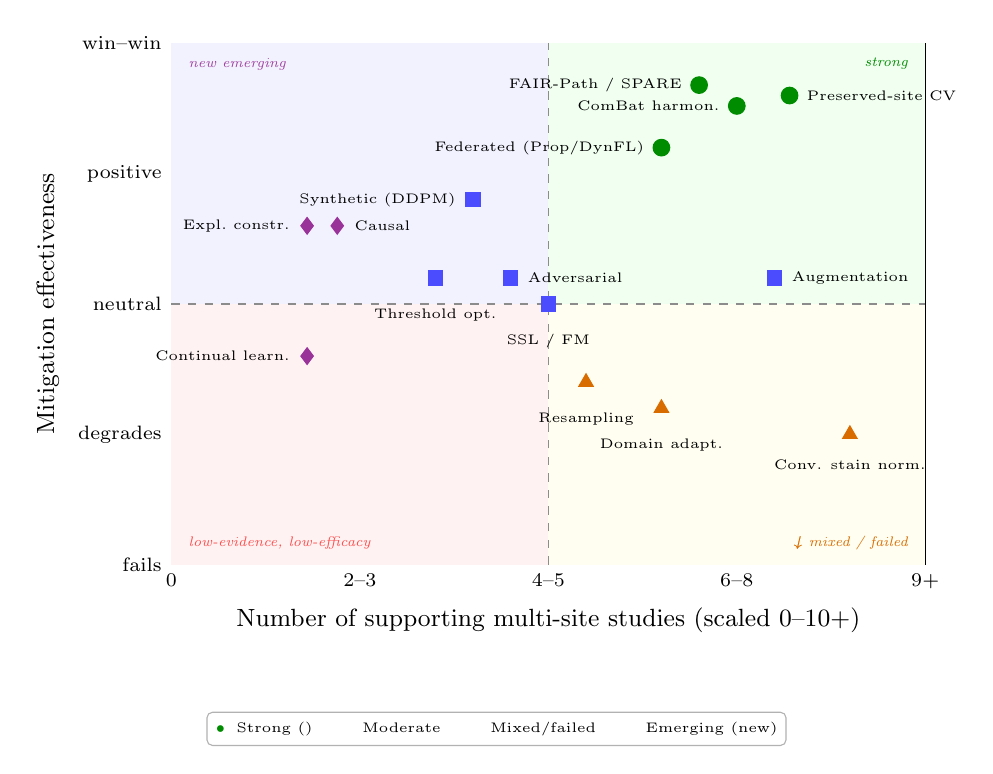
\begin{tikzpicture}[font=\scriptsize]
    \begin{axis}[
        width=0.92\linewidth, height=8.2cm,
        xmin=0, xmax=1, ymin=0, ymax=1,
        xlabel={Number of supporting multi-site studies (scaled 0--10$+$)},
        ylabel={Mitigation effectiveness},
        xlabel style={font=\small}, ylabel style={font=\small},
        xtick={0.0,0.25,0.5,0.75,1.0},
        xticklabels={0,2--3,4--5,6--8,9$+$},
        ytick={0,0.25,0.5,0.75,1.0},
        yticklabels={fails,degrades,neutral,positive,win--win},
        tick label style={font=\scriptsize},
        major grid style={draw=black!10},
        grid=major,
        clip=false,
      ]
      % Quadrant shading
      \path[fill=green!6]  (axis cs:0.5,0.5) rectangle (axis cs:1,1);
      \path[fill=yellow!6] (axis cs:0.5,0)   rectangle (axis cs:1,0.5);
      \path[fill=blue!5]   (axis cs:0,0.5)   rectangle (axis cs:0.5,1);
      \path[fill=red!5]    (axis cs:0,0)     rectangle (axis cs:0.5,0.5);
      \draw[dashed, black!45] (axis cs:0.5,0) -- (axis cs:0.5,1);
      \draw[dashed, black!45] (axis cs:0,0.5) -- (axis cs:1,0.5);

      % Strong (green circles)
      \addplot[only marks, mark=*, mark size=3pt,
               color=green!55!black]
        coordinates {(0.82,0.90) (0.75,0.88) (0.70,0.92) (0.65,0.80)};
      % Moderate (blue squares)
      \addplot[only marks, mark=square*, mark size=2.6pt,
               color=blue!70]
        coordinates {(0.80,0.55) (0.45,0.55) (0.50,0.50)
                     (0.40,0.70) (0.35,0.55)};
      % Mixed (orange triangles)
      \addplot[only marks, mark=triangle*, mark size=3pt,
               color=orange!85!black]
        coordinates {(0.90,0.25) (0.55,0.35) (0.65,0.30)};
      % Emerging (purple diamonds)
      \addplot[only marks, mark=diamond*, mark size=3pt,
               color=violet!80]
        coordinates {(0.22,0.65) (0.18,0.65) (0.18,0.40)};

      % Labels
      \node[anchor=west,font=\tiny] at (axis cs:0.83,0.90) {Preserved-site CV};
      \node[anchor=east,font=\tiny] at (axis cs:0.74,0.88) {ComBat harmon.};
      \node[anchor=east,font=\tiny] at (axis cs:0.69,0.92) {FAIR-Path / SPARE};
      \node[anchor=east,font=\tiny] at (axis cs:0.64,0.80) {Federated (Prop/DynFL)};
      \node[anchor=west,font=\tiny] at (axis cs:0.81,0.55) {Augmentation};
      \node[anchor=west,font=\tiny] at (axis cs:0.46,0.55) {Adversarial};
      \node[anchor=north,font=\tiny] at (axis cs:0.50,0.46) {SSL / FM};
      \node[anchor=east,font=\tiny] at (axis cs:0.39,0.70) {Synthetic (DDPM)};
      \node[anchor=north,font=\tiny] at (axis cs:0.35,0.51) {Threshold opt.};
      \node[anchor=north,font=\tiny] at (axis cs:0.90,0.22) {Conv. stain norm.};
      \node[anchor=north,font=\tiny] at (axis cs:0.55,0.31) {Resampling};
      \node[anchor=north,font=\tiny] at (axis cs:0.65,0.26) {Domain adapt.};
      \node[anchor=west,font=\tiny] at (axis cs:0.23,0.65) {Causal};
      \node[anchor=east,font=\tiny] at (axis cs:0.17,0.65) {Expl.\ constr.};
      \node[anchor=east,font=\tiny] at (axis cs:0.17,0.40) {Continual learn.};

      % Quadrant labels
      \node[font=\tiny\itshape,text=green!55!black,anchor=north east]
        at (axis cs:0.99,0.99) {\checkmark\ strong};
      \node[font=\tiny\itshape,text=violet!75,anchor=north west]
        at (axis cs:0.01,0.99) {new emerging};
      \node[font=\tiny\itshape,text=orange!85!black,anchor=south east]
        at (axis cs:0.99,0.01) {\textdownarrow\ mixed / failed};
      \node[font=\tiny\itshape,text=red!70,anchor=south west]
        at (axis cs:0.01,0.01) {low-evidence, low-efficacy};
    \end{axis}
    % Legend
    \node[draw=black!30, rounded corners=2pt, inner sep=3pt,
          font=\tiny, fill=white, align=left]
         at ([yshift=-1.1cm]current bounding box.south)
         {\begin{tabular}{@{}l@{\hspace{4pt}}l@{\hspace{14pt}}
                          l@{\hspace{4pt}}l@{\hspace{14pt}}
                          l@{\hspace{4pt}}l@{\hspace{14pt}}
                          l@{\hspace{4pt}}l@{}}
          \textcolor{green!55!black}{$\bullet$} & Strong (\checkmark) &
          \textcolor{blue!70}{$\blacksquare$} & Moderate &
          \textcolor{orange!85!black}{$\blacktriangle$} & Mixed/failed &
          \textcolor{violet!80}{$\blacklozenge$} & Emerging (new) \\
         \end{tabular}};
  \end{tikzpicture}
  \caption{\textbf{Mitigation-method effectiveness against evidence
           base across the 78 included studies.}  Each marker
           is one of the $16$ method families catalogued in
           Table~\ref{tab:mitigation_summary}.  The vertical axis
           encodes the typical reported effect (win--win fairness
           gain without accuracy loss, positive, neutral, degraded,
           or failed); the horizontal axis encodes the size and
           breadth of the empirical base (number of supporting
           multi-site or multi-cohort studies, scaled).
           \emph{Upper-right quadrant}~(\checkmark~\textbf{strong}):
           preserved-site CV, ComBat feature harmonisation, FAIR-Path
           and SPARE fairness-aware learning, and federated learning
           (Prop-FFL, DynamicFL) deliver fairness gains ($61$--$91\%$
           disparity reduction) with preserved or improved
           accuracy~\citep{howard2021site, murchan2024combat,
           lin2025contrastive, xu2026spare, hosseini2023proportionally,
           zhang2025dynamicfl, huang2025knowledge}.
           \emph{Upper-left}~(new/emerging):
           causal, explanation-constraint, and continual-learning
           methods show promise but are backed by ${\leq}3$ studies
           each.
          \emph{Lower-right}~(\textdownarrow~mixed/failed despite adoption):
          stain normalization, class resampling, and classical domain
          adaptation are widely used yet fail to close cross-batch
          or demographic gaps (cross-batch AUROC range $0.74\!\to\!0.52$
          worst case even after conventional Macenko/Reinhard/Vahadane normalization;
           CORAL/IRM/GroupDRO ineffective on WILDS-CAMELYON17)~\citep{
           komen2024batch, lin2025stain, voon2023evaluating,
           koh2021wilds}.}
  \label{fig:mitigation_grid}
\end{figure}

% ── 3.3  Mitigation Methods ──────────────────────────────────
\subsection{Mitigation Methods}
\label{sec:results:mitigation}

\label{sec:results:mit:stain}%
\label{sec:results:mit:augmentation}%
Having documented the extent of bias and the under-reporting of fairness metrics, we now synthesise evidence on mitigation strategies. Across the 16 mitigation method families synthesised below
(Table~\ref{tab:mitigation_summary}; Figure~\ref{fig:mitigation_grid}),
evidence quality varies considerably. Preprocessing and data-level methods show mixed effectiveness. Stain normalization illustrates this variability: across 15+ studies evaluating six computational stain normalization methods (Reinhard, Macenko, SPCN, ACD, StainGAN, StainNet), no significant accuracy improvement was found~\citep{voon2023evaluating}, with cross-batch AUROC remaining near chance (0.52--0.61) even after Macenko, Reinhard, and Vahadane normalization~\citep{komen2024batch, lin2025stain}. Image-level color correction appears insufficient to remove batch effects from deep features~\citep{komen2024batch} or close fairness gaps (graded "Mixed (workflow) / Failed (fairness)" in Table~\ref{tab:mitigation_summary}: improves workflow but fails to remove site-level confounding). However, advanced computational methods show promise: attention-guided residual stain normalization achieves SSIM~0.9663 (4.6\% improvement over StainGAN) while better preserving tissue structure~\citep{madusanka2025structure}, and MultiStain-CycleGAN reduces domain-classifier accuracy to 0.672 while preserving tumour-classification performance~\citep{hetz2024multi}. Distinct from computational methods, physical calibration slides---a laboratory quality-control approach---improved cross-site Gleason~$\kappa$ from 0.35--0.44 to 0.45--0.74~\citep{ji2025physical}, and computational stain normalization improved inter-pathologist Gleason risk-group agreement while reducing diagnosis time from 50~s to 33~s in a 407-WSI multi-institutional study ($p < 0.001$)~\citep{cazaniga2024not}. In summary, conventional stain normalization methods alone (Macenko, Reinhard, Vahadane) fail to remove site-level confounding and close fairness gaps, while advanced methods improve image quality and workflow efficiency but require further validation for fairness outcomes.

Data augmentation shows moderate efficacy across 20+ studies. RandAugment
outperformed manual baselines on CAMELYON17 (AUROC 0.827 vs.\ 0.799,
$p < 0.001$)~\citep{faryna2024automatic}, while AugmentHist increased color
dispersion by 81\% and boosted AUROC by up to
21.7\%~\citep{franchet2024bias}. Combined normalization--augmentation
pipelines outperform either approach alone~\citep{franchet2024bias}, though augmentation
alone does not address demographic or institutional
bias~\citep{howard2021site}. Dataset curation and resampling yield similarly mixed results. Preserved-site CV exposed inflated performance for $35.7$\% of
features~\citep{howard2021site}, while quality-control tools such as GrandQC
prevent artefact-driven bias from entering training
pipelines~\citep{weng2024grandqc}. Class-level SMOTE improved balanced
accuracy by up to 3.4\%~\citep{rezama2018imbalanced}, though
demographic-level resampling proved
ineffective~\citep{soltan2024challenges}. ComBat harmonisation substantially reduced site-prediction AUROC from
above 0.95 to approximately 0.5 while preserving MSI-status prediction
(AUROC 0.669~$\to$~0.669, $p = 0.95$) and improving BRAF prediction
on external data (0.622~$\to$~0.691)~\citep{murchan2024combat}.
Pan-cancer analyses confirm pervasive site effects at the feature
level~\citep{chen2022pan}, and feature-selection methods show promise: multi-objective selection via
NSGA-II reduced institution-classification accuracy by 36--40\% while
improving external-validation F1 from 79.83\% to
85.90\%~\citep{bidgoli2022bias}, while ranking-loss instance sequestering
cut hospital-classification accuracy from 73\% to
41.6\%~\citep{mazaheri2023ranking}.

\label{sec:results:mit:ssl}%
Domain adaptation and adversarial methods yield mixed results across 10+ studies. Successful domain adaptation applications include AIDA, which improved balanced accuracy from 64.65\% to
78.82\%~\citep{asadiaghbolagh2024learning}; K-TOP MIL, which achieved 95.89\%~AUROC
for multi-domain ovarian cancer classification~\citep{ahmed2025robust}; and adversarial DA, which improved
prostate-cancer AUROC from 0.657 to
0.745~\citep{ren2019unsupervised}. CycleGAN-based stain transfer
improved cross-center AUROC from 0.57--0.84 to
0.92--0.98~\citep{nerrienet2023standardized}. However, invariant risk minimisation approaches have fared worse: CORAL, IRM, and
Group DRO all failed on WILDS-Camelyon17~\citep{koh2021wilds}, and visually
convincing CycleGAN translations do not reliably reduce domain
shift~\citep{vasiljevic2022cyclegan}. Adversarial debiasing shows moderate evidence across 8+ studies. Gradient reversal suppresses site
features effectively, though the approach is sensitive to hyperparameters and
may remove causally relevant
information~\citep{lafarge2019learning, otalora2019staining}. DANN
combined with color augmentation most frequently achieves the best
cross-domain results~\citep{otalora2019staining}.

Learning-based approaches show promise across several paradigms. Self-supervised and foundation-model approaches produce moderately promising results across 5+ studies: SimCLR pretrained
on 57 histopathology datasets improved macro F1 from 66.7\% to
77.0\%~\citep{ciga2023self}, and foundation models reduce but do not
eliminate batch effects (TSS-prediction accuracy 62--78\% when fine-tuned; $>$90\% when frozen with linear probes)~\citep{komen2024batch}.
Virchow trained on 1.5\,M WSIs, for example, shows residual TSS-specific
biases~\citep{vorontsov2024foundation}. FLEX reduced NSCLC-TYPE fairness gap from 0.041 to 0.016 while
improving OOD AUROC by 6.4--7.2\%~\citep{huang2025knowledge}, and a systematic benchmark of
11~public pathology foundation models across 22~clinical tasks from
3~medical centers found that pretraining dataset composition is the
primary driver of downstream task performance~\citep{campanella2025clinical}. Fairness-aware learning offers the strongest and most consistent evidence across 10+ studies. FAIR-Path
mitigated 88.5--91.1\% of baseline disparities across 20~cancer
types~\citep{lin2025contrastive}, while SPARE improved minority-group
accuracy by 3.7--5.8\%~\citep{xu2026spare}. Equitable training
frameworks integrate group-level performance
constraints~\citep{shi2025equitable}, though Group DRO failed on
WILDS~\citep{koh2021wilds}. Federated learning demonstrates strong cross-site equity gains across 6+ studies. Prop-FFL reduced
inter-hospital variance from 32.54 to
10.00~\citep{hosseini2023proportionally}, while DynamicFL achieved 87.37\%
versus 78.08\% baseline~\citep{zhang2025dynamicfl}. FL outperformed
centralised training on external melanoma data (AUROC 0.913 versus
0.905, $p < 0.001$)~\citep{haggenmuller2024federated}, and federated learning with differential privacy preserves diagnostic
accuracy at competitive AUROC~\citep{lu2022federated, adnan2022federated}.
FL for invasive carcinoma detection achieved competitive accuracy,
$F_1$, and AUROC across hospitals~\citep{agbley2022federated}; see~\citep{shukla2025federated} for a comprehensive review.

Post-hoc and generative methods offer complementary strategies with moderate evidence. Post-hoc threshold adjustment across 4+ studies shows that group-specific
thresholds can achieve equalised odds but require attribute labels at
deployment~\citep{soltan2024challenges, sufian2024mitigating}, while
conformal prediction provides distribution-free coverage
guarantees~\citep{bhattacharyya2025conformal}. Synthetic data generation via conditional diffusion models shows moderate promise across 4+ studies:
conditional DDPMs yielded a 48.5\% relative fairness improvement and
3.2\% absolute gain over color augmentation on
CAMELYON17~\citep{ktena2024generative}, and GAN synthesis for
underrepresented Gleason grades improved grading accuracy by
15--32\%~\citep{vanbooven2025mitigating}. Several emerging approaches warrant further investigation, each backed by three or fewer studies. Causal survival models
equalise prediction across
sites~\citep{correamedero2024causal}. ECGL reduced equalised-odds
difference by 73\%~\citep{shabazian2025joint}, and LRP heatmaps guide
targeted augmentation (AUROC~$+5\%$)~\citep{hagele2020resolving}. Other nascent directions include
uncertainty calibration for MIL via label
smoothing~\citep{park2025uncertainty}; continual learning fairness
remains unpredictable~\citep{cecconi2024fairness}.

% ─── Performance--fairness trade-offs ─────────────────────
\label{sec:results:tradeoffs}%
Methods targeting root causes of bias, specifically batch effects, shortcut features, or site-specific artefacts, consistently achieve win--win outcomes (Table~\ref{tab:tradeoffs}). FLEX improved OOD AUROC by
6--7\% while reducing fairness gaps by
61\%~\citep{huang2025knowledge}. FAIR-Path resolved 88.5--91.1\% of
disparities with no AUROC drop~\citep{lin2025contrastive}, and ComBat
eliminated site signal while preserving clinical
predictions~\citep{murchan2024combat}. NSGA-II feature selection
improved external F1 by 6.1\% while reducing institutional
bias~\citep{bidgoli2022bias}. By contrast, surface-level methods such as stain
normalization, along with overly noisy interventions such as aggressive
differential privacy, fail to improve fairness and may degrade
performance~\citep{voon2023evaluating, lu2022federated}. No single debiasing method significantly outperformed
ERM across all settings~\citep{zong2023medfair}; instead, Pareto-optimal model
selection consistently achieved the best balance. With fewer than
13\% of studies reporting dual-axis (performance + fairness) results,
routine adoption of Pareto-frontier analysis represents a critical priority.

%% ─── Trade-off summary table ─────────────────────────────
\begin{table}[!ht]
  \centering
  \caption{Quantitative summary of reported performance--fairness
           trade-offs.  ``Accuracy~$\Delta$'' indicates the change in
           the primary performance metric (AUROC, F1, or accuracy);
           ``Fairness~$\Delta$'' indicates the change in the primary
           disparity or equity metric.
           $\uparrow$~improvement;
           $\downarrow$~degradation;
           $\approx$~no significant change.}
  \label{tab:tradeoffs}
  \small
  \begin{tabularx}{\linewidth}{@{}l l l l c@{}}
    \toprule
    \textbf{Method} & \textbf{Study} &
      \textbf{Accuracy $\Delta$} & \textbf{Fairness $\Delta$} &
      \textbf{Pattern} \\
    \midrule
    FLEX (info.\ bottleneck)
      & \citet{huang2025knowledge}
      & OOD AUROC $\uparrow$6--7\%
      & Gap $\downarrow$61\%
      & Win--win \\
    FAIR-Path (contrastive)
      & \citet{lin2025contrastive}
      & AUROC $\approx$
      & Disparity $\downarrow$88.5\%
      & Win--win \\
    SPARE (reweighting)
      & \citet{xu2026spare}
      & Acc $\uparrow$3.7--5.8\%
      & FATE $\uparrow$
      & Win--win \\
    ComBat (harmonisation)
      & \citet{murchan2024combat}
      & MSI AUROC $\approx$
      & Site AUROC $\to$0.5
      & Win--win \\
    NSGA-II (feature sel.)
      & \citet{bidgoli2022bias}
      & F1 $\uparrow$6.1\%
      & Inst.\ acc $\downarrow$36\%
      & Win--win \\
    Cond.\ DDPM (synthetic)
      & \citet{ktena2024generative}
      & $\uparrow$3.2\% vs aug.
      & $\uparrow$48.5\%
      & Win--win \\
    DynamicFL
      & \citet{zhang2025dynamicfl}
      & 87.4\% vs 78.1\%
      & Consistent
      & Win--win \\
    FL (melanoma)
      & \citet{haggenmuller2024federated}
      & Holdout $\downarrow$4.5\%
      & OOD $\uparrow$0.8\%
      & Moderate \\
    Pseudo-Label (CL)
      & \citet{cecconi2024fairness}
      & AUROC $\downarrow$9\,pp
      & Gender EO 0.001
      & Moderate \\
    Conventional stain normalization
      & \citet{voon2023evaluating}
      & BAcc $\approx$
      & Bias $\approx$
      & Failed (fairness) \\
    Demographic resampling
      & \citet{soltan2024challenges}
      & Acc $\approx$
      & Bias $\approx$
      & Failed \\
    \bottomrule
  \end{tabularx}
\end{table}

Approximately 70.5\% (95\% CI: 59.7--79.5\%) of studies lack multi-site external validation. Standard
cross-validation inflates AUROC by approximately 0.069~\citep{howard2021site}, and
open-source implementations remain rare~\citep{koh2021wilds,
weng2024grandqc}. Demographic metadata is sparsely available across the 39~audited public datasets: race/ethnicity in 28.2\% (95\% CI: 16.5--43.8\%), sex in 25.6\% (95\% CI: 14.6--41.1\%), and age in 23.1\% (95\% CI: 12.6--38.3\%). Six fairness-critical fields (genetic ancestry, Fitzpatrick skin tone, intersectional identifiers, preferred language, protected-attribute flags, and data-quality scores) show zero availability~\citep{norori2021addressing, montezuma2025unbiased}. Reporting guideline adherence is similarly limited: no
study explicitly cites CLAIM or TRIPOD+AI compliance, and the STARD-AI
protocol remains the only framework directly addressing AI
diagnostic reporting~\citep{sounderajah2021stardai}. Addressing these gaps requires structured
adoption of existing frameworks with mandatory fairness-specific items,
including disaggregated performance reporting, dataset provenance documentation, and bias-mitigation
documentation~\citep{chen2023algorithmic, yang2024survey,
chinta2025aidriven}.

\label{sec:results:summary}%
Bias in histopathology AI is multifactorial and co-occurring
(Section~\ref{sec:results:taxonomy}), yet fairness measurement remains
the exception rather than the norm
(Section~\ref{sec:results:metrics}). Only 19.2\% of studies report any
fairness metric, and 5.1\% report worst-group
accuracy~\citep{soltan2024challenges, xu2026spare}. Effective mitigation strategies exist but remain under-adopted. Methods with strong empirical
support include preserved-site CV~\citep{howard2021site}, ComBat
harmonisation~\citep{murchan2024combat}, fairness-aware learning
(FAIR-Path~\citep{lin2025contrastive}, SPARE~\citep{xu2026spare},
FLEX~\citep{huang2025knowledge}), and federated
learning~\citep{hosseini2023proportionally, zhang2025dynamicfl}. These approaches achieve
simultaneous performance and equity gains, whereas widely used but
demonstrated-ineffective techniques such as stain normalization and standard
domain adaptation~\citep{voon2023evaluating, koh2021wilds} persist in practice.
Reproducibility deficits, including limited code sharing, narrow dataset
concentration, demographic metadata gaps, and negligible
reporting-guideline adherence, constitute the most pressing structural
barrier to progress~\citep{norori2021addressing, sounderajah2021stardai,
chinta2025aidriven}.
